\section{Three-Class Classification}
\lb{sec:3class}

One of the caveats of the analysis with two classes is that there are associated sources, which do not belong to AGN or PSR classes. These have the labels: unk, spp, glc, snr, gal, sbg, GAL, sfr, bin, SNR, HMB, LMB, css, PWN, pwn, hmb, SFR, BIN, lmb, NOV.%
%\footnote{\dima{write a complete list of labels in the OTHER class}}
We collect all these associated sources, which do not belong to AGN and PSR classes into a new class, which we label as ``OTHER''.
Since in two-class classification we train algorithm to classify sources only into AGN and PSR classes, OTHER sources are also classified as either AGN or PSR.
This introduces a bias in the estimates of the number of AGNs and pulsars among unassociated sources.
One possibility to correct this bias is to assume that the fractions of OTHER sources among associated and unassociated sources are the same (Equation (\ref{eq:other_correction})).
This correction can be applied for the total number of sources or for the number of sources in some window of parameters,
e.g., in a flux bin or in a range of latitudes and longitudes.
This is a straightforward calculation but it has some limitations. In particular, it implicitly assigns equal probabilities to all AGNs (and all PSRs) to belong to the OTHER class.
For a small range of parameters the variance of this estimate can be very large due to small number of associated OTHER sources in this parameter range.

In this section we discuss the construction of probabilistic catalogs with multi-class classification (three-class classification in our case).
We start with the construction of the probabilistic catalog based on 3FGL by adding the class ``OTHER'', which includes all associated sources without AGN or PSR associations: there are 108 such sources in 3FGL.
We use the same 11 features as in the 2-class classification: the only difference is that we use cos(GLON) instead of GLON.
The reason is that LR and NN methods have a significantly worse performance than RF and BDT methods when we use GLON,
but, as we show below, all four methods have comparable accuracy when we use cos(GLON).
This can be due to discontinuity in the GLON variable. 
We perform optimization of the meta-parameters for the four ML algorithms with the 3 classes.


\begin{figure}[h]
\center
%\hspace*{-1cm}
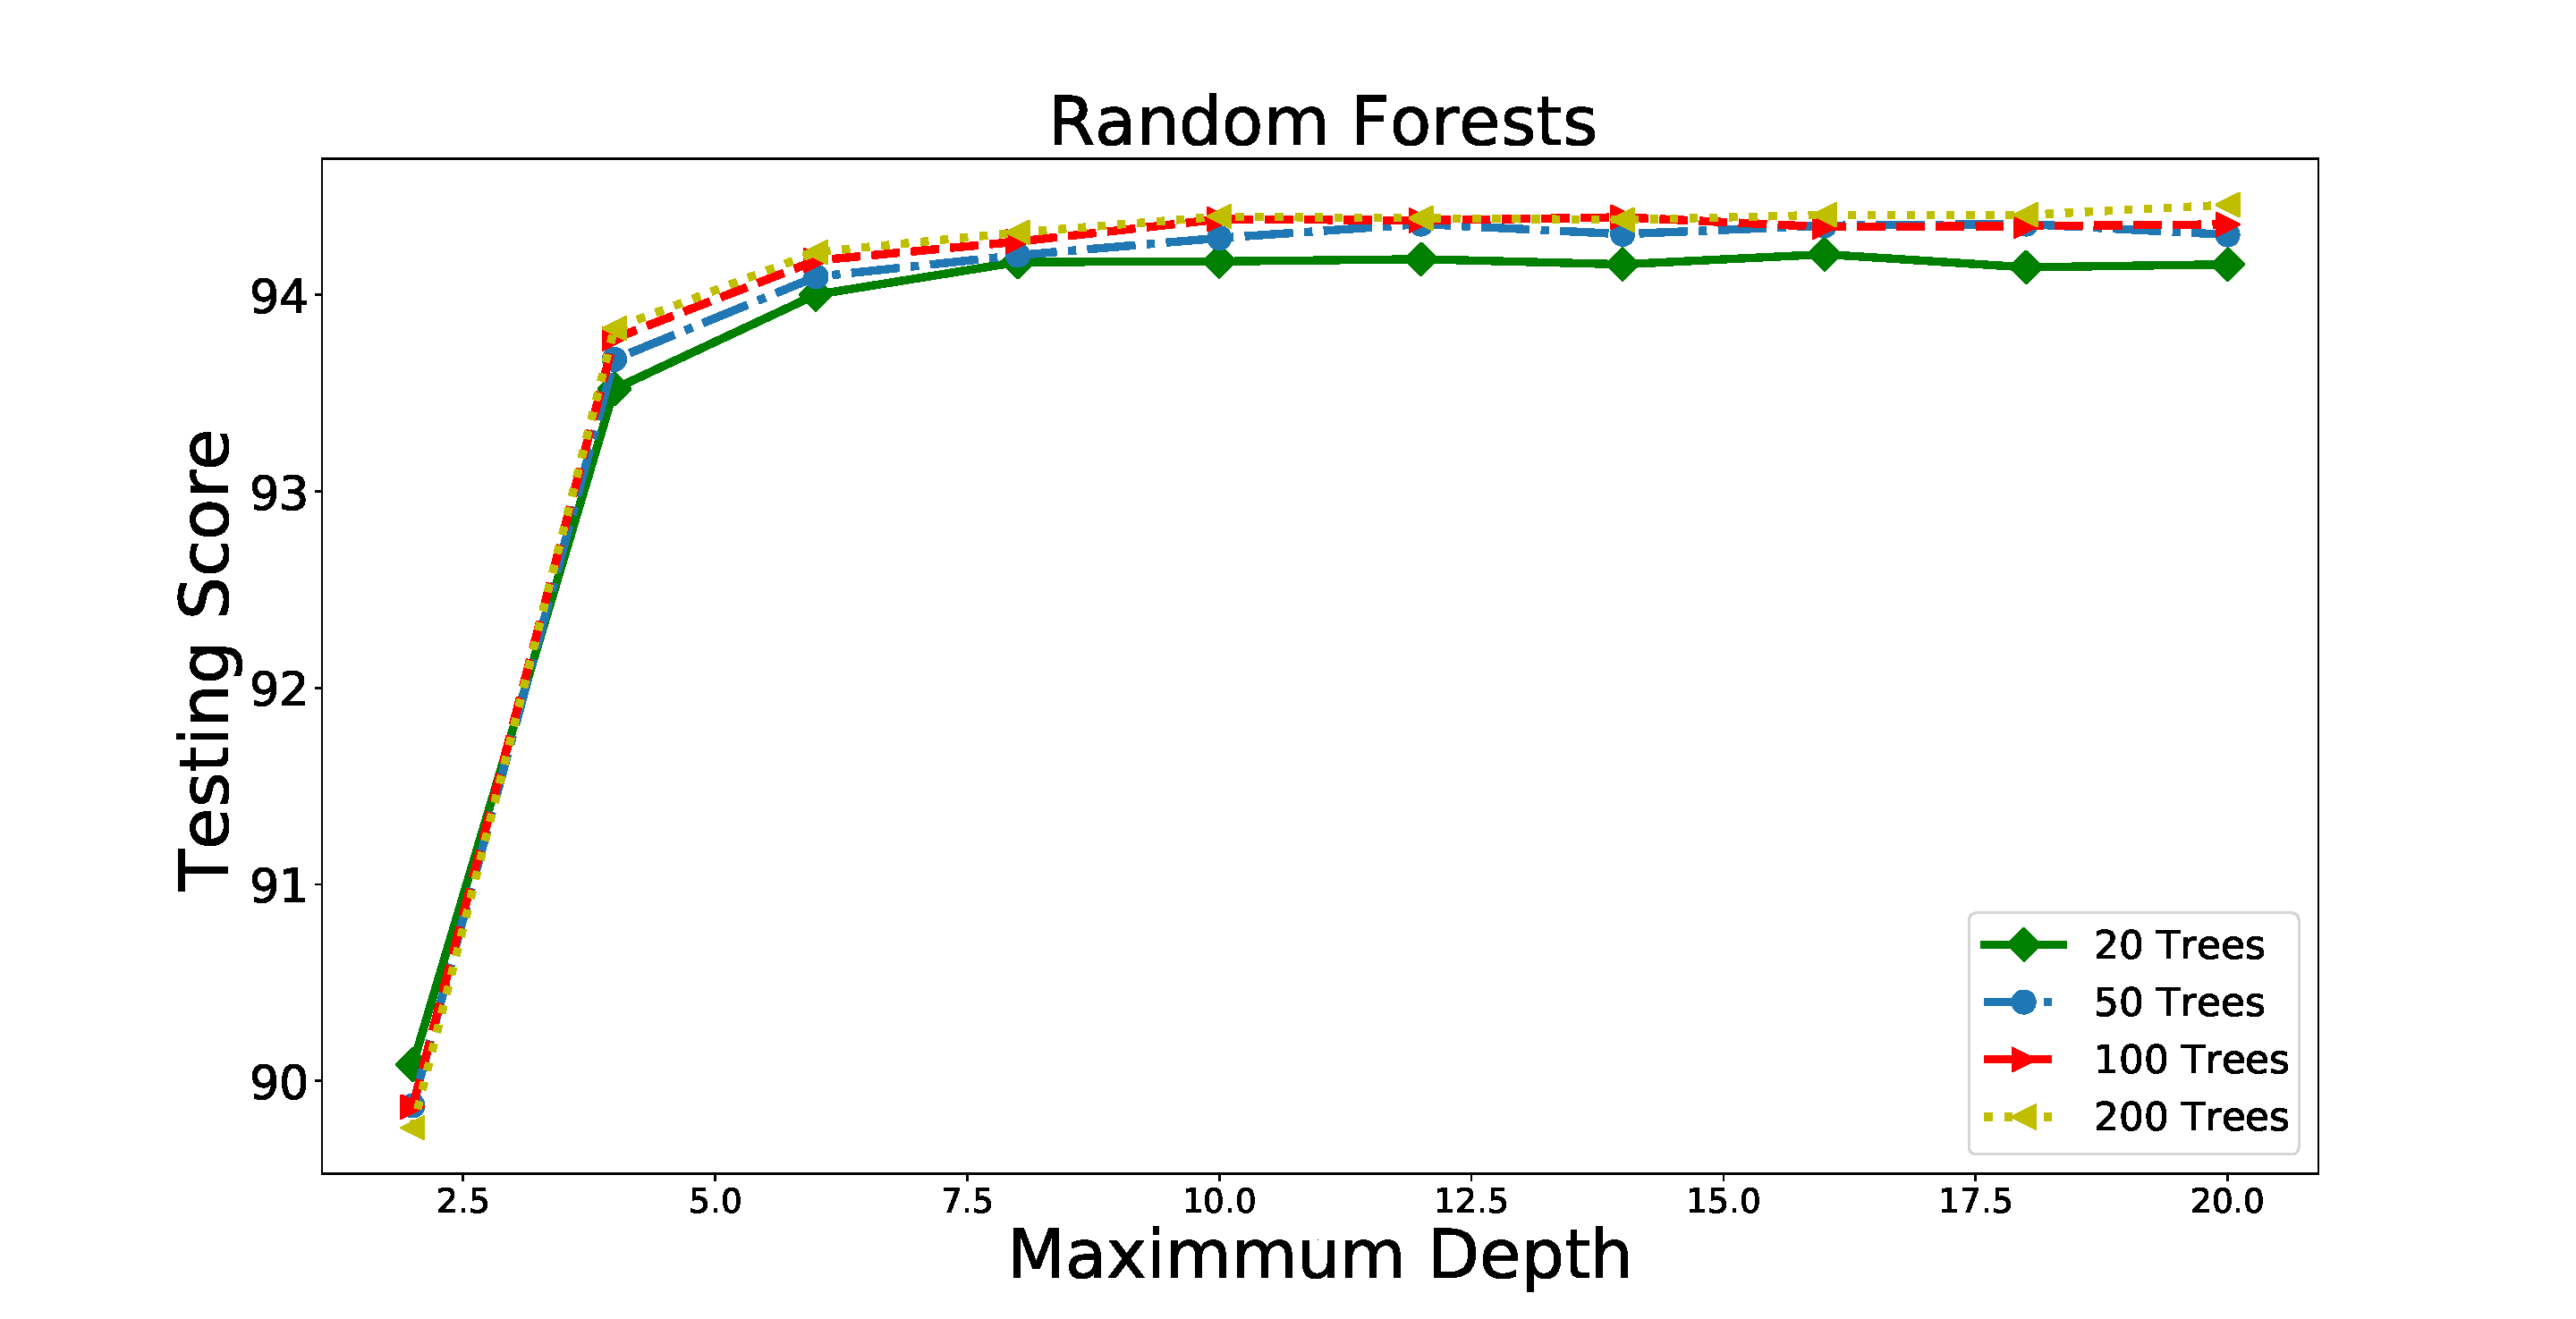
\includegraphics[width=0.5\textwidth]{plots/rf_train_multi.pdf}\\
%\hspace*{-1cm}
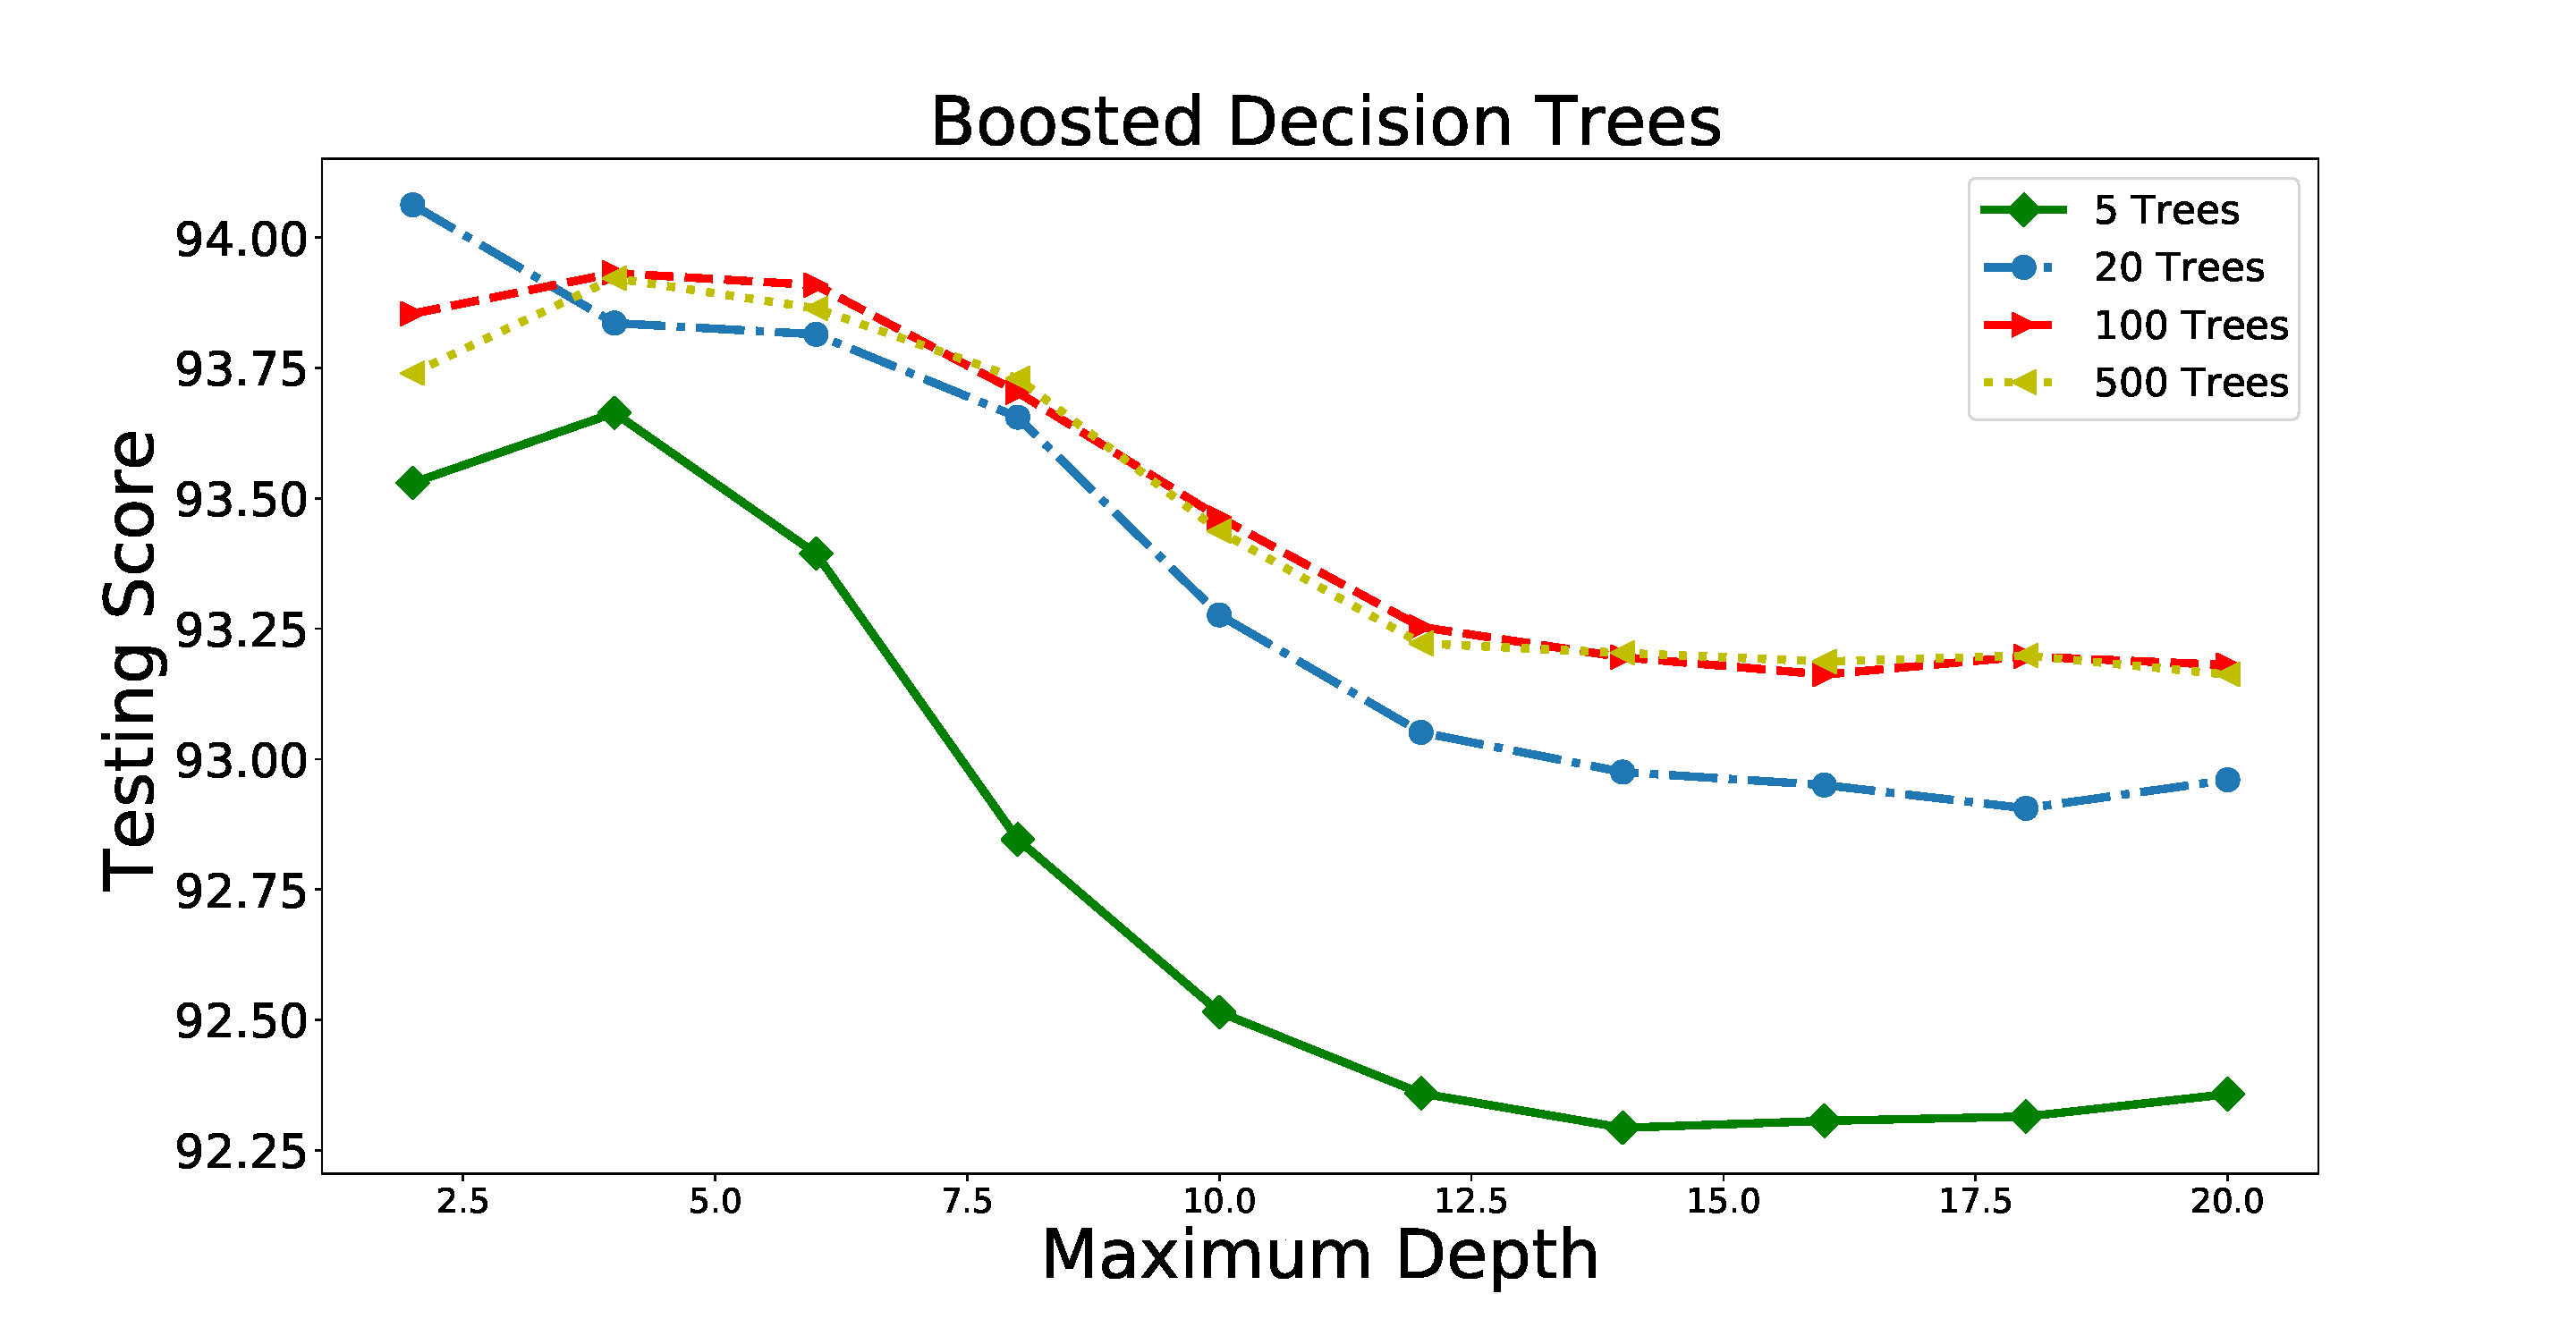
\includegraphics[width=0.5\textwidth]{plots/bdt_train_multi.pdf}
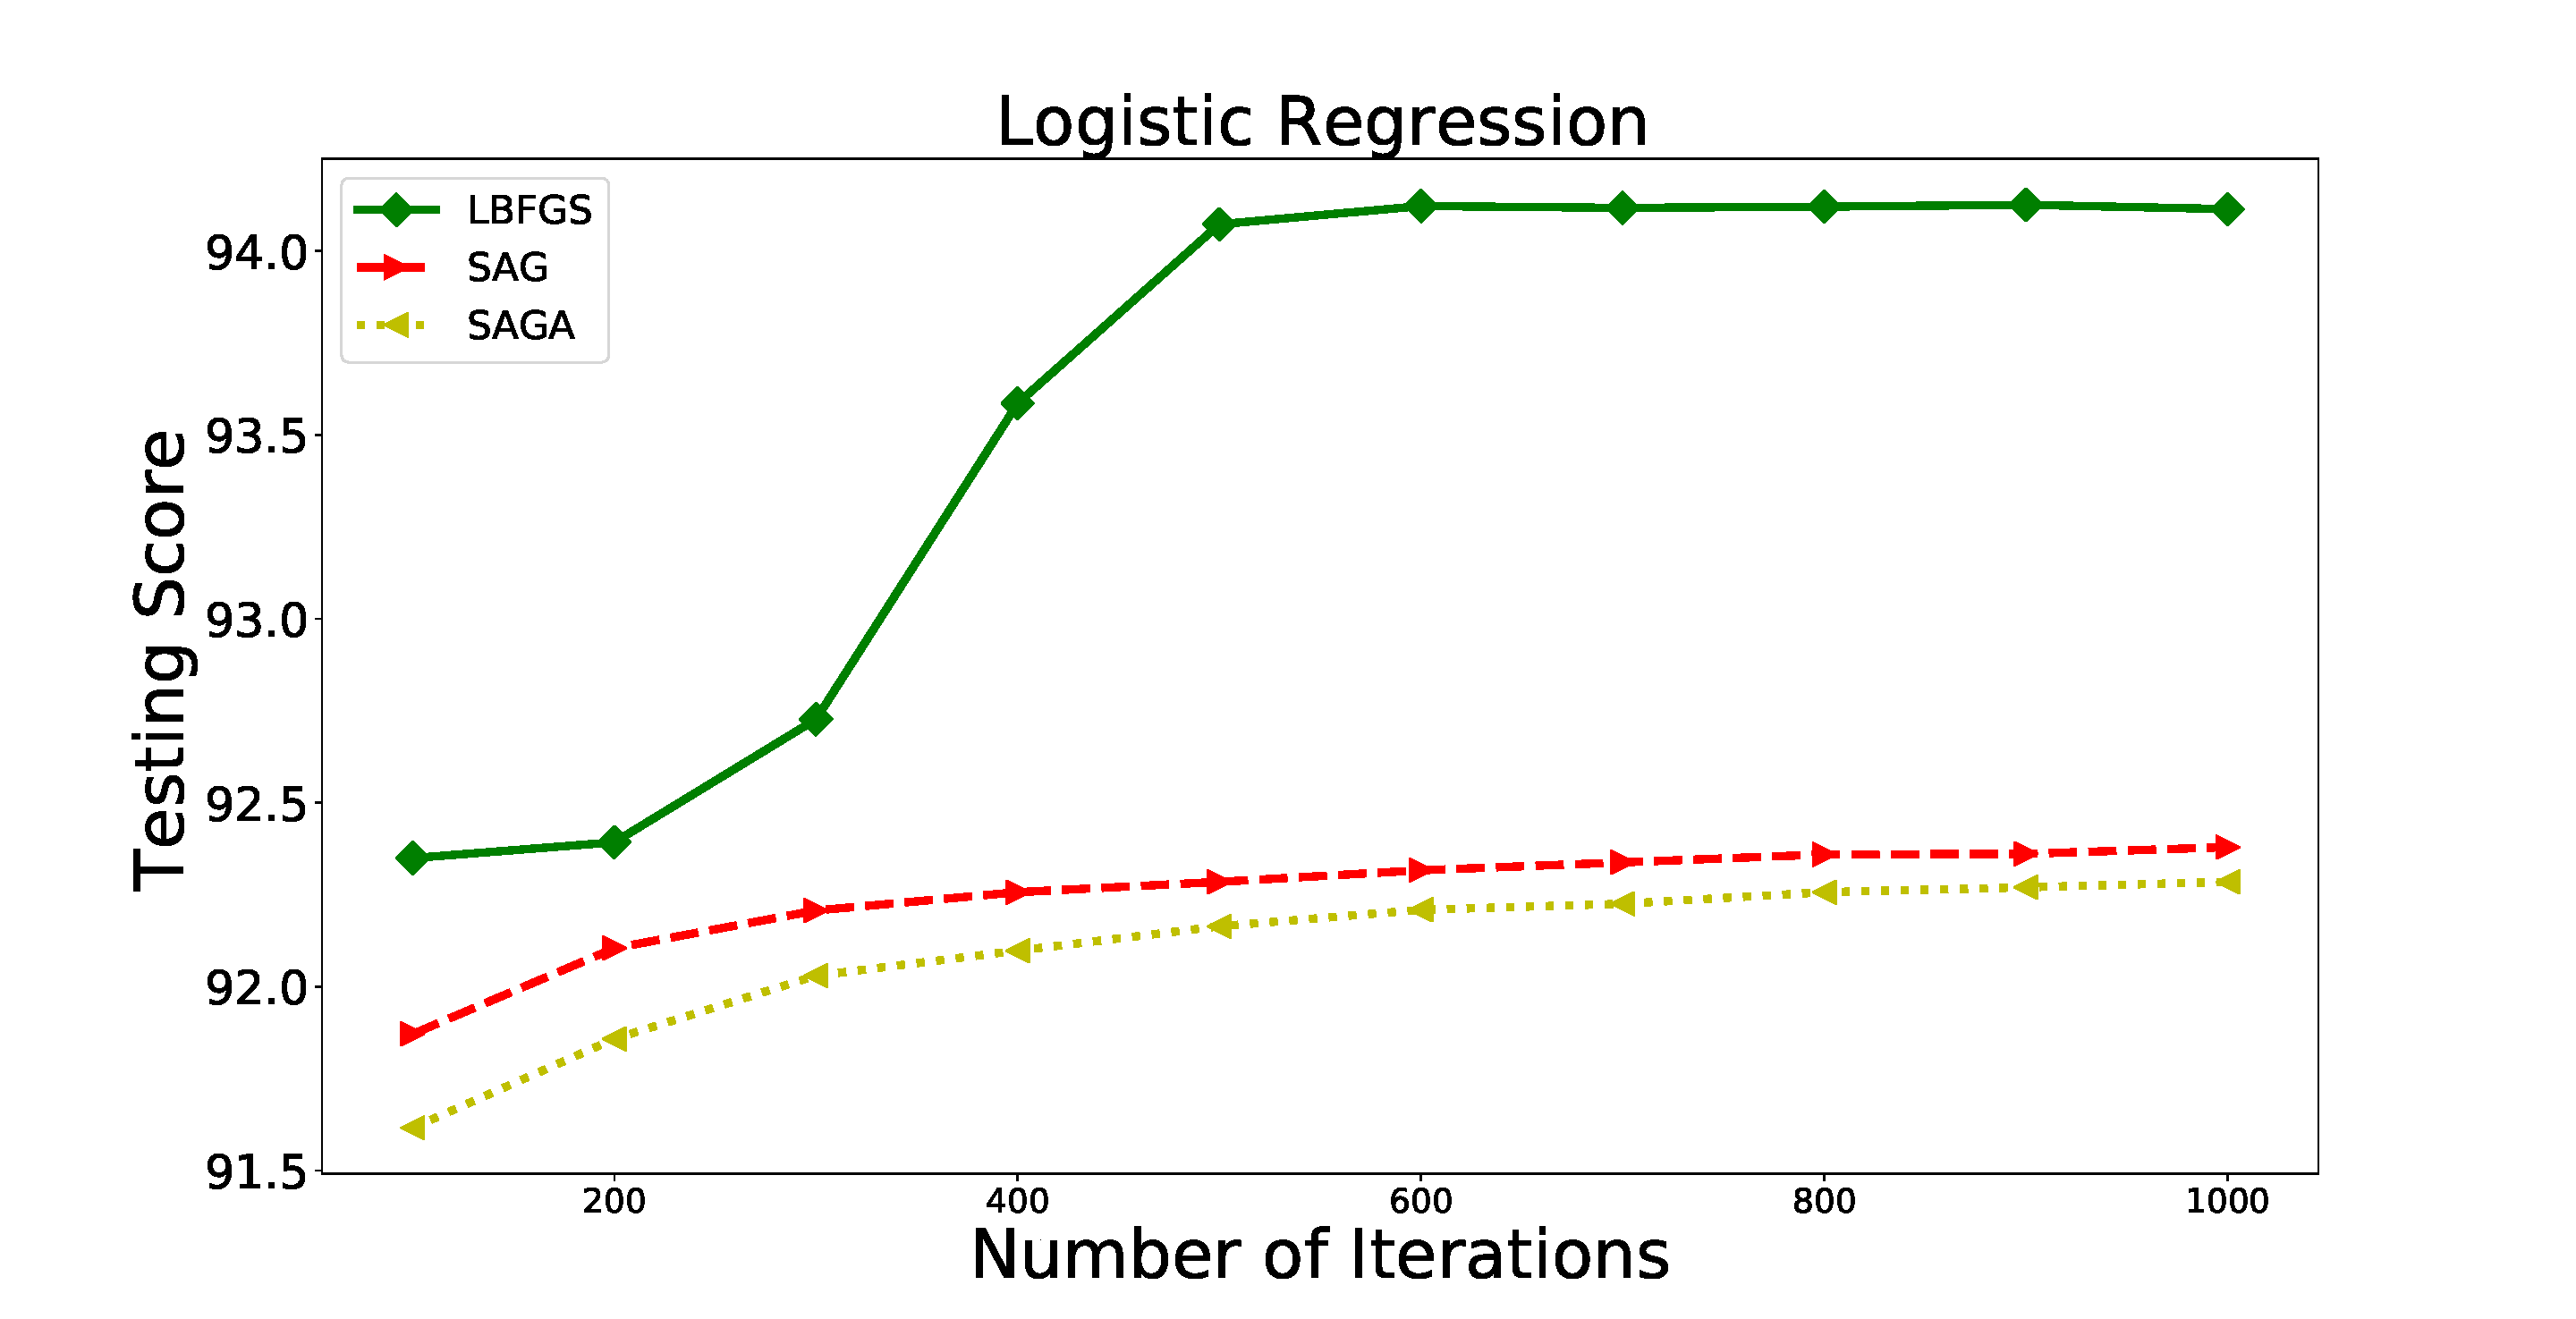
\includegraphics[width=0.5\textwidth]{plots/lr_train_multi.pdf}
\caption{Accuracy for the 3-class classification with RF, BDT and LR  methods. LR doesn't have Liblinear solver here, since Liblinear cannot handle multinomial loss.
%\dima{Why there are four lines and only 3 labels in the LR plot? It's strange that there is such a large difference between
%LBFGS and other lines.}
}
\label{fig:tree_multi}
\end{figure}

\begin{figure}[h]
\center
%\hspace*{-1cm}
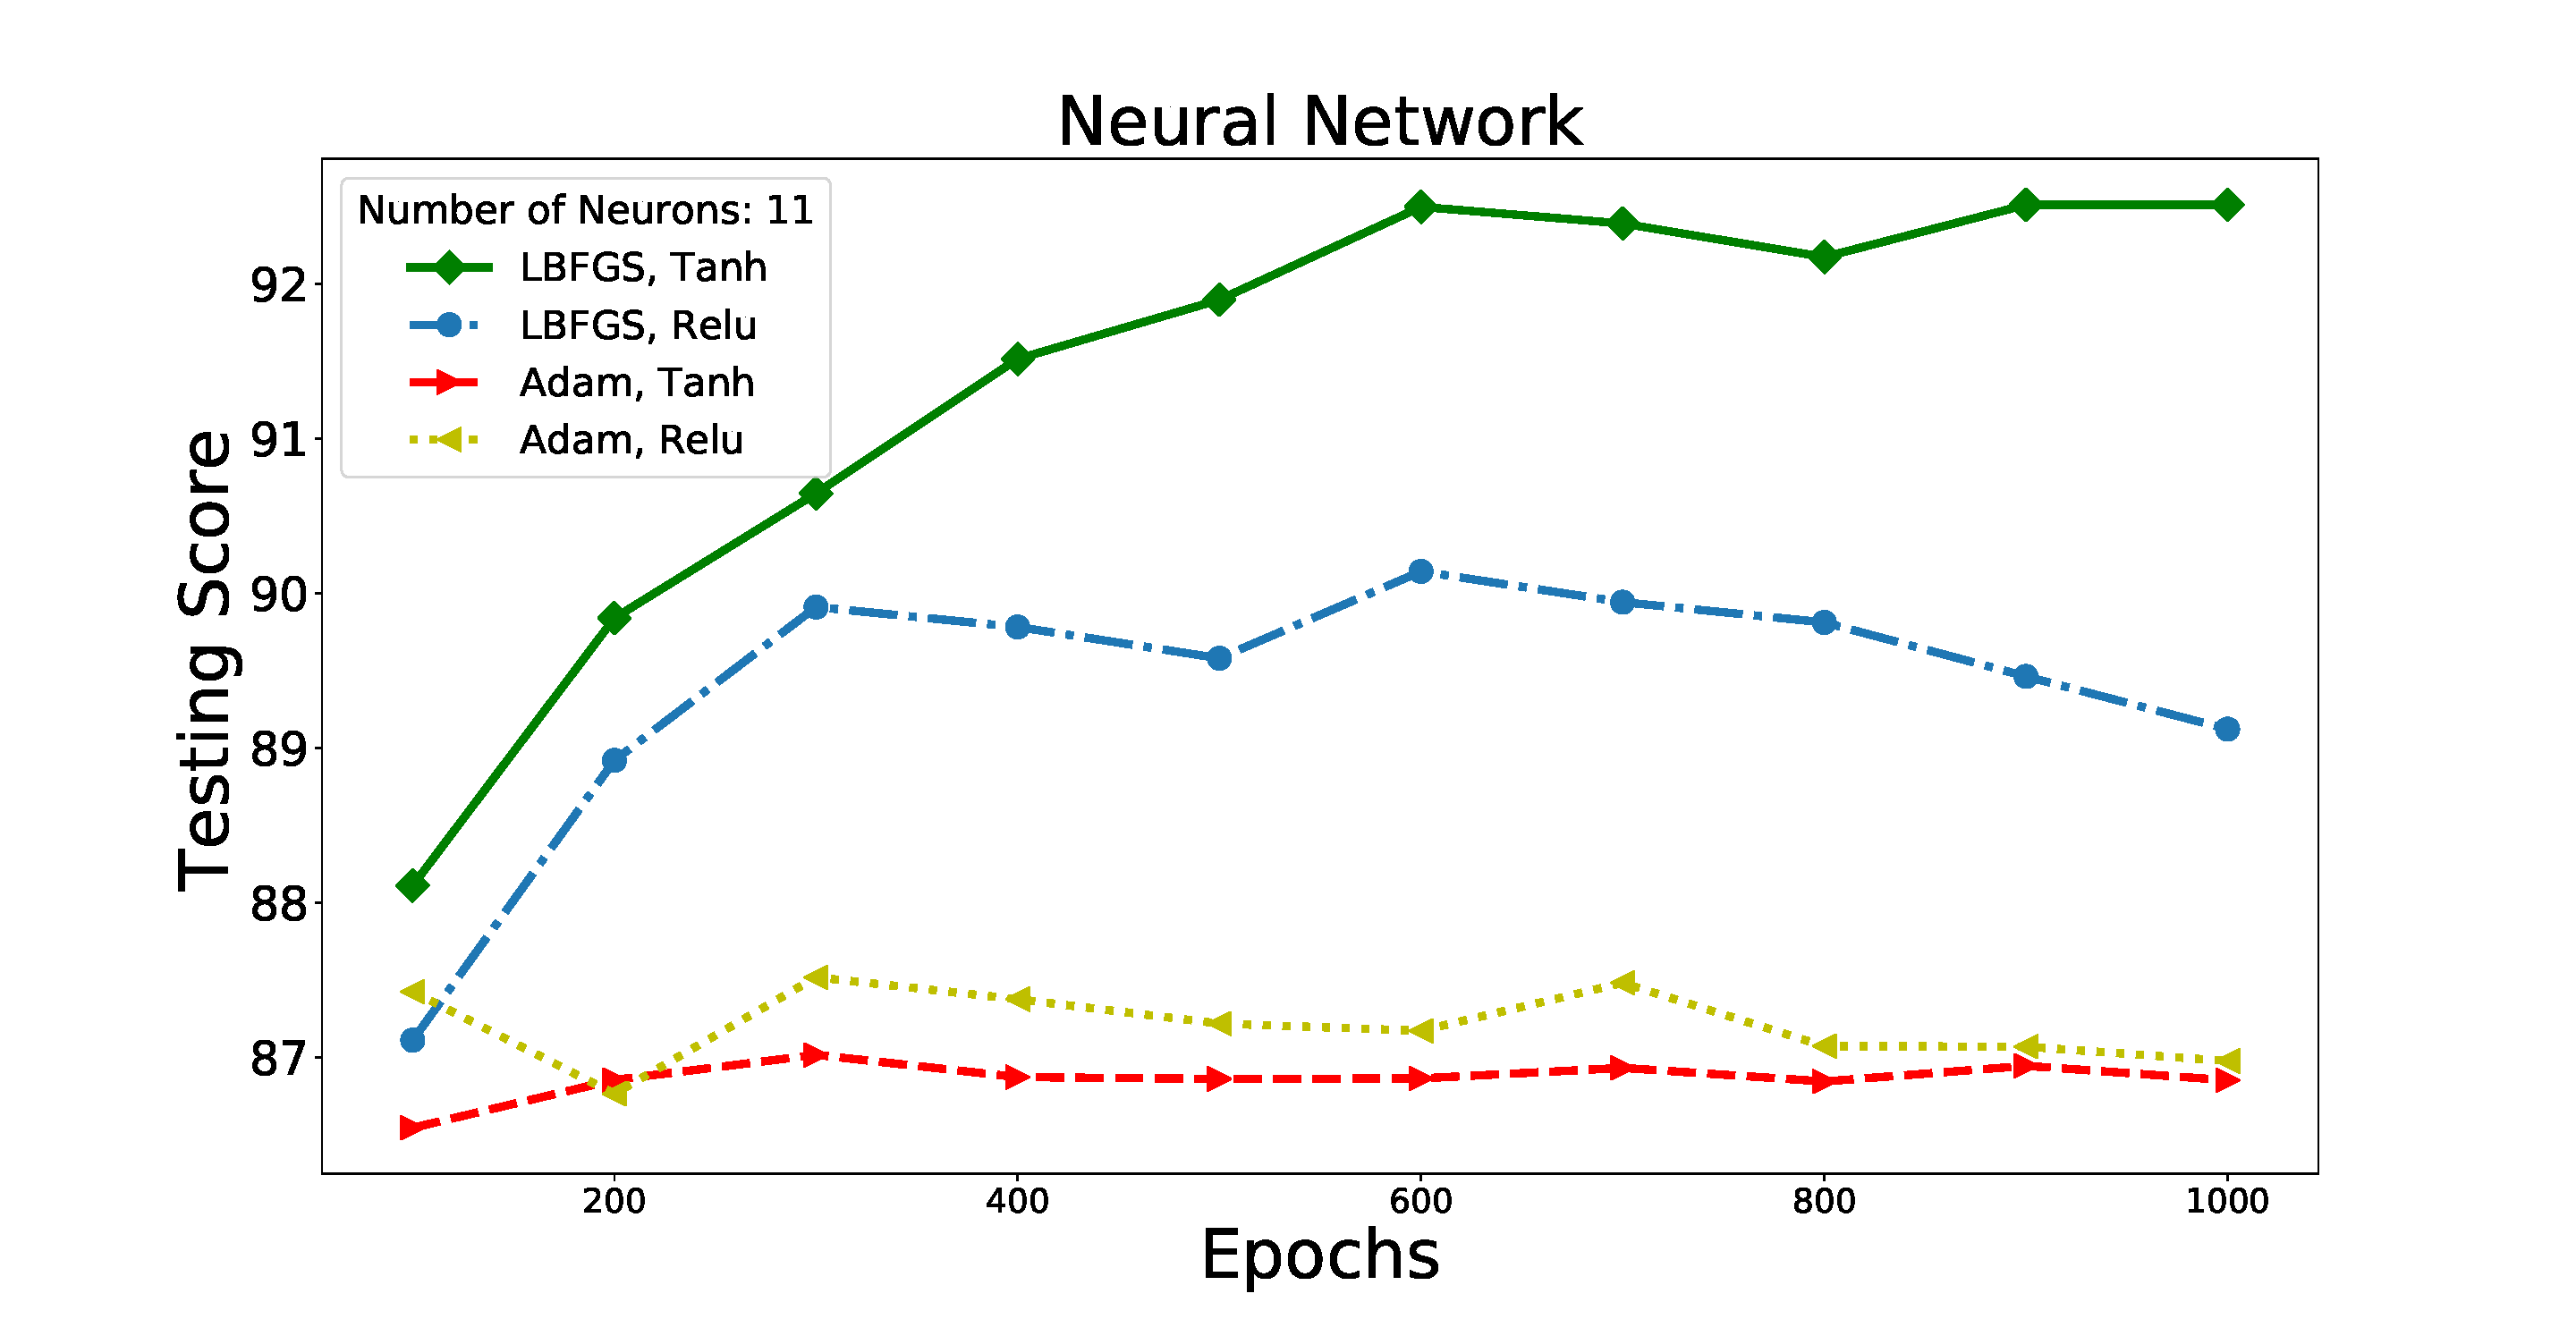
\includegraphics[width=0.5\textwidth]{plots/nn_epoch_train_multi.pdf}\\
%\hspace*{-1cm}
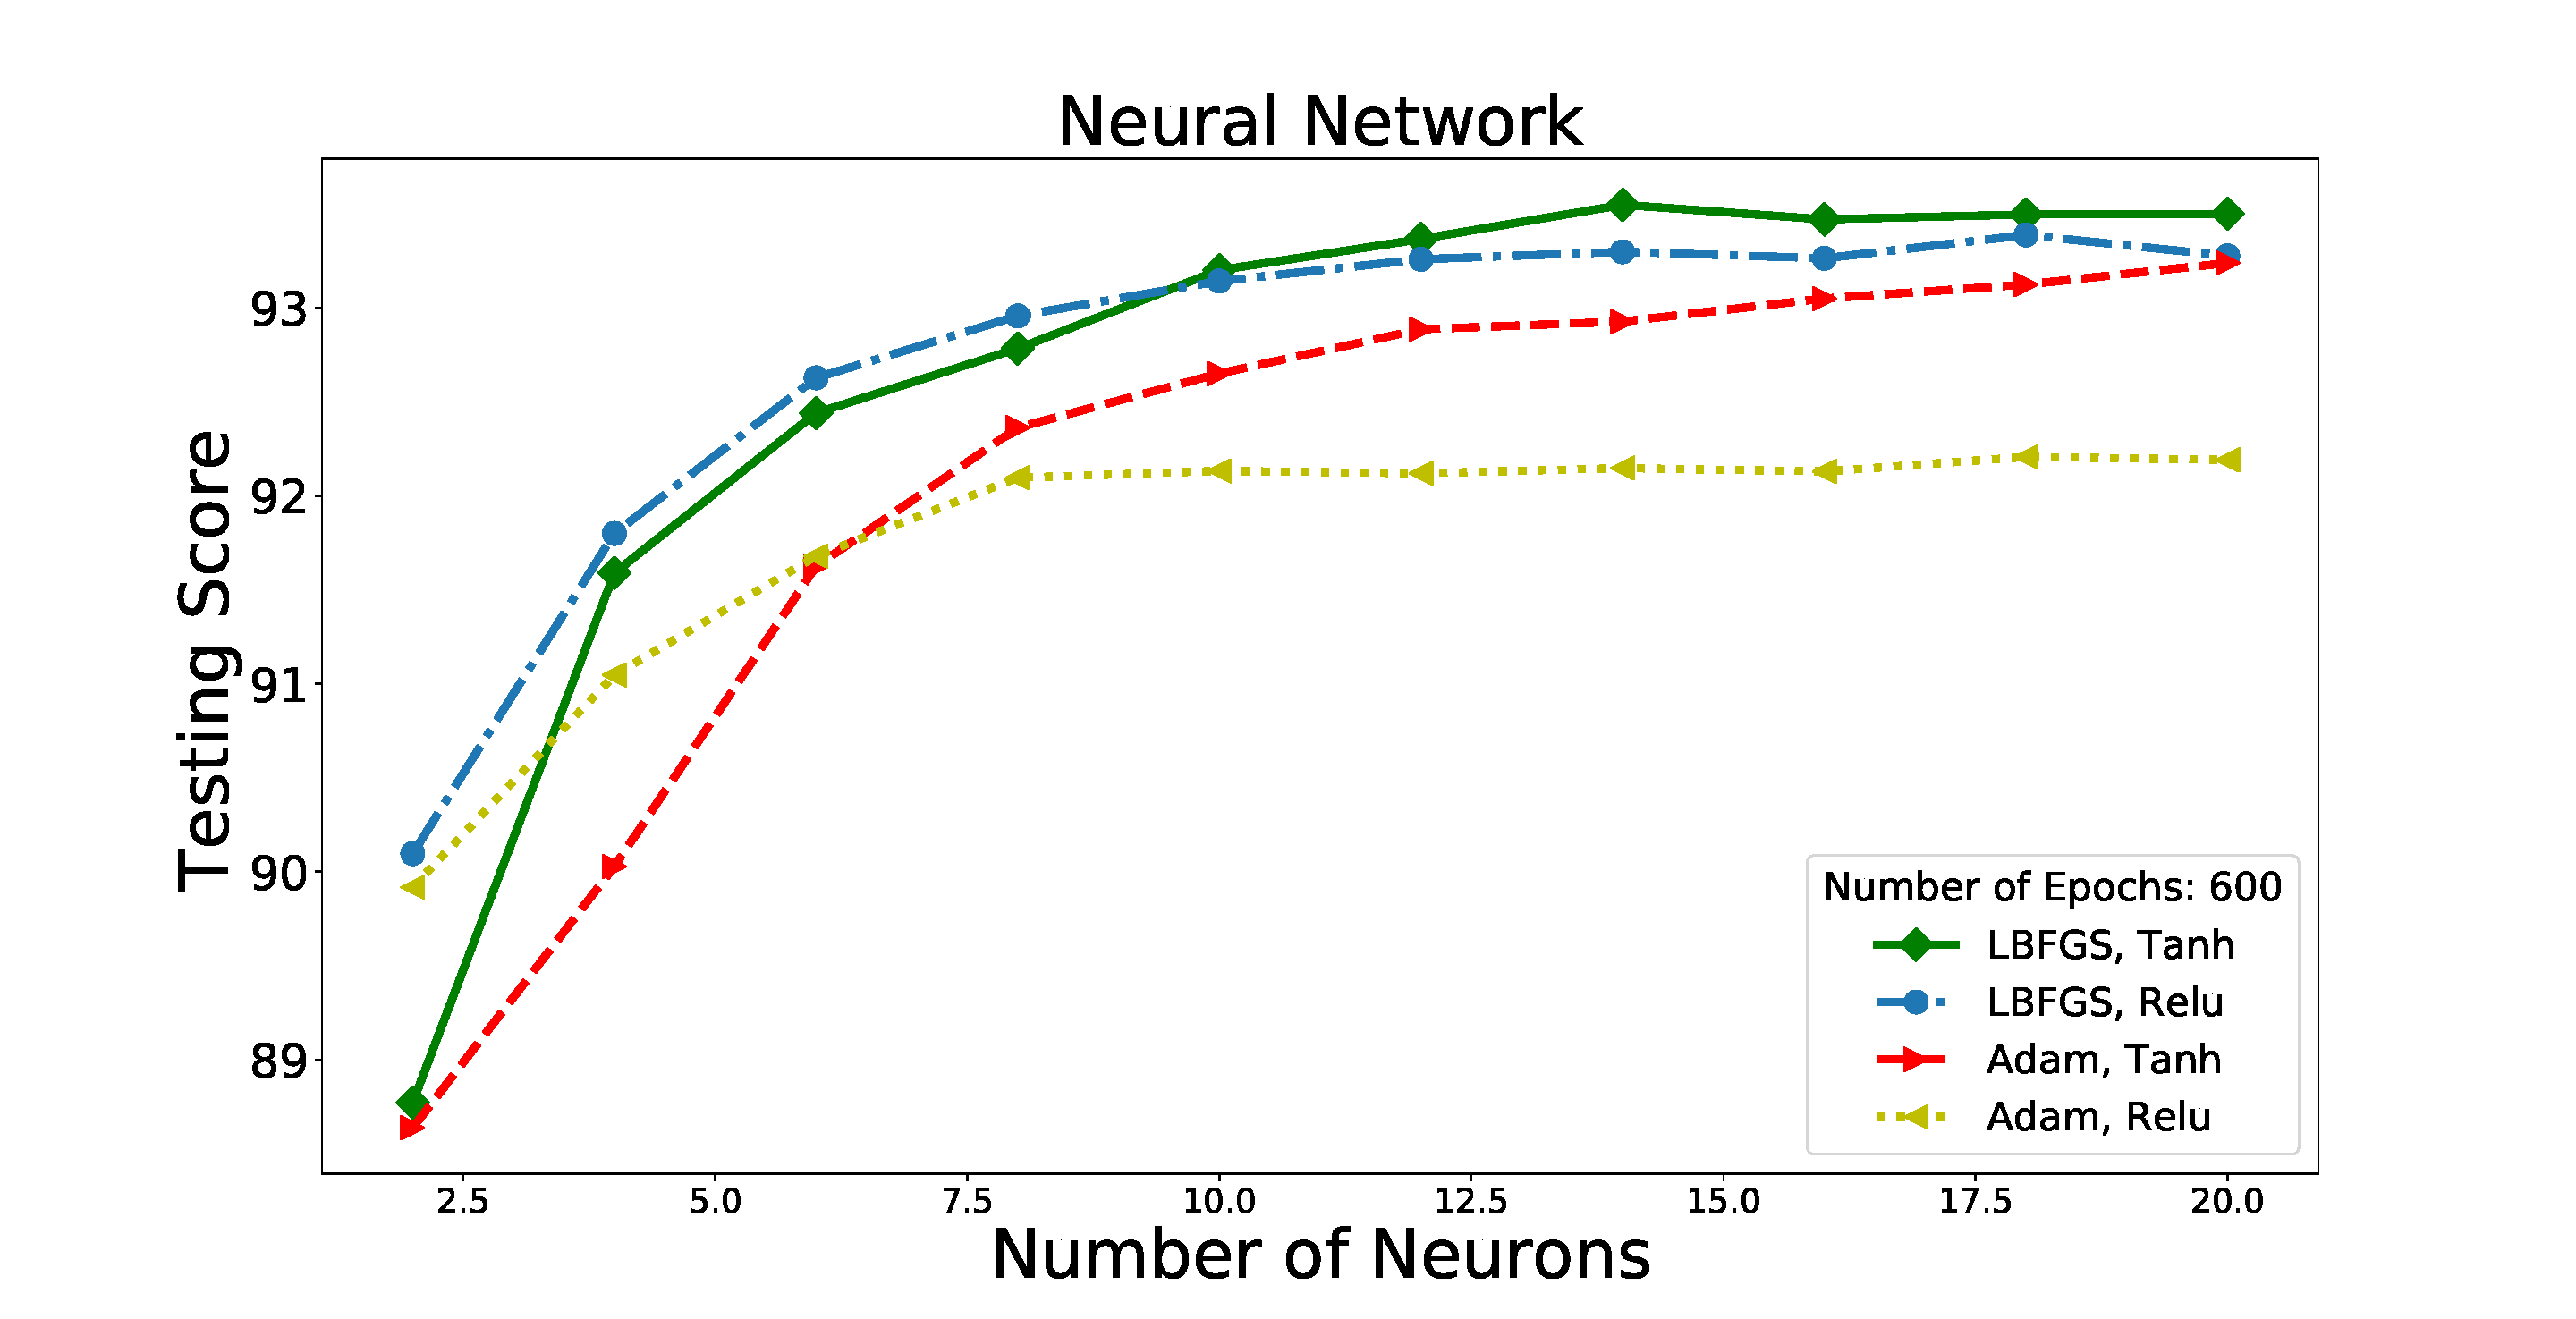
\includegraphics[width=0.5\textwidth]{plots/nn_neuron_train_multi.pdf}
\caption{Accuracy of the NN classification as a function of the number of epochs and of the number of neurons
 for the 3-class classification. 
% \dima{Can you check the Adam calculation? It's strange that the difference is so large: 
% the top panel has accuracy of 91\% for 11 neurons and 600 epochs, while the bottom panel has only 87\% accuracy for the same parameters.}
 }
\label{fig:nets_multi}
\end{figure}


The dependence of accuracy on meta-parameters of the algorithms is shown in Figures \ref{fig:tree_multi} and \ref{fig:nets_multi}.
We see that for the tree-based algorithms, the optimal parameters are similar to the 2-class classification, i.e., 50 trees with depth 6 for RF and 100 trees with depth 2 for BDT 
provide close to optimal performance at a minimal cost in complexity (depth of the trees).
The main difference for NN and LR algorithms is that more steps are needed for convergence for both normal and oversampled cases. This is why we opt for 600 epochs for NN and 500 iterations for LR instead of 300 epochs and 200 iterations respectively in the two-class case. %\dima{Why do we use 600 epochs if in LBFGS case the convergence happens already for 100 epochs?}
For NN, the accuracy stops increasing above about 10 neurons in the hidden layer (in the following we use 11 neurons for classification: the same as in the two-class case).

For oversampling, we use the oversampling factors $\sqrt{\frac{\text{\# AGN}}{\text{\# PSR}}}$ and $\sqrt{\frac{\text{\# AGN}}{\text{\# OTHER}}}$ for PSR and OTHER classes respectively (instead of $\frac{\text{\# AGN}}{\text{\# PSR}}$ and $\frac{\text{\# AGN}}{\text{\# OTHER}}$ oversampling factors in the 2-class case).
The reason for a smaller oversampling factors is to avoid overweighting the relatively small OTHER class.

The accuracies of our chosen models for classification of the 3FGL sources are presented in Table \ref{tab:selected_algs_multi}.
As in the 2-class case, the accuracies are averaged over 1000 realizations of splitting the data into training and testing samples.
We notice that accuracies presented in Table \ref{tab:selected_algs} are calculated relative to AGN and PSR classes only, if we take into account that all OTHER sources
are misclassified in this case, then the testing accuracy is reduced by about 5\% (the fraction of OTHER sources in associated source in 3FGL),
while the accuracy of comparison with 4FGL-DR2 is reduced by about 10\% (there are 37 unassociated sources in 3FGL with OTHER class associations in 4FGL-DR2,
while there are in total 339 unassociated sources in 3FGL with associations in 4FGL-DR2).
Thus the testing accuracy of 93-94\% in Table \ref{tab:selected_algs_multi} provides at least a 1-2\% improvement over the accuracy in Table \ref{tab:selected_algs},
after taking into account the misclassification of OTHER sources in the 2-class case.
The corresponding improvement for the accuracy of classification of unassociated sources in 3FGL with 4FGL-DR2 associations is more than 5\%.




%In this section we discuss the multi-class method\footnotemark\footnotetext{Multi here refers to any non-binary number of classes}. Instead of only using sources which had AGN and PSR as their classification we added 108 sources in the 3FGL catalog which have a classification not falling under AGN or PSR. We gave them a classification of 'OTHER'. We ran our codes again, first to find the optimum parameters as was done in section 2. The only differences here are that we took the cosine of the galactic longitude and the oversampling was done with the square root of the fraction of AGNs with the PSR or OTHER classifications. Therefore, for oversampling, the number of PSRs and OTHERs were multiplied by $\sqrt{\frac{\text{|AGN|}}{\text{|PSR|}}}$ and $\sqrt{\frac{\text{|AGN|}}{\text{|OTHER|}}}$ respectively. We chose these weights so as to not oversample and bias our methods too much. This is effectively clear for instance if we would go to even higher classes and the number of data points shall become smaller. 

%Figure \ref{fig:tree_multi} and \ref{fig:nets_multi} shows our results.The tree based methods show the same behaviour as before and therefore we keep the same parameters for our final models. For Neural Networks and Logistic regression the behaviour is also the same but the optimal parameters are found to be 600 and 500 epochs instead of 300 and 200 respectively. We keep the same number of neurons as before for the neural network.


\begin{table}[!h]
\hspace{-0.2cm}
\resizebox{0.47\textwidth}{!}{
    \tiny
  \centering
    \renewcommand{\tabcolsep}{0.4mm}
\renewcommand{\arraystretch}{1.6}

%\hspace{-3mm}
    \begin{tabular}{|c|c|c|c|c|c|c|}
    \hline
    Algorithm&Parameters &  Testing&Std. Dev.& Comparison with \\
    & & Accuracy & & 4FGL DR-2 Accuracy \\
    \hline
    RF & 50 trees, max depth 6  &93.96&0.85& 88.92  \\
    RF\_O &   &94.38&0.76& 87.87 \\
    \hline %\midrule   -> aakash do you mean this?
    BDT & 100 trees, max depth 2    &   93.72&0.83&87.20 \\
%    \hline %\midrule   -> aakash do you mean this?
%    BDT & 200 trees, max depth 2    &   95.8  \\
    BDT\_O &     &   93.83&0.80& 86.69 \\
    \hline
    NN & 600 epochs, 11 neurons, LBFGS & 93.17&1.05& 86.39\\
    NN\_O &&  92.51 &1.34& 83.97\\
    \hline
    LR & 500 iterations, LBFGS solver & 93.93&0.88& 87.65 \\
    LR\_O &   &93.01&0.96& 85.59 \\
    \hline
    \end{tabular}}
    \vspace{2mm}
    \caption{Testing accuracy of the four selected algorithms for 3-class classification of 3FGL sources and comparison with associations in the 4FGL-DR2 catalog. 
    ``\_O'' denotes training with oversampling.}
    \label{tab:selected_algs_multi}
\end{table}


\begin{table}[!h]
\resizebox{0.3\textwidth}{!}{
    \tiny
 %  \centering
    \renewcommand{\tabcolsep}{0.3mm}
\renewcommand{\arraystretch}{1.5}

    \begin{tabular}{| l |c|c|c|c|}
    \hline
    Catalog & AGN & PSR & OTHER & Mixed \\
    \hline
    3FGL & 585 & 53 & 69  &  301 \\
    4FGL-DR2 & 736 & 64 & 271  &  587 \\
    \hline
     
    \end{tabular}}
    \vspace{0.2cm}
    \caption{Expected number of AGNs, pulsars, and other sources as well as sources with mixed classifications
    among the unassociated 3FGL and 4FGL-DR2 sources derived with the 3-class classification.}
    \label{tab:prediction_3class}
\end{table}



The 3-class classification of 4FGL-DR2 sources is performed similar to the 3-class classification of the 3FGL sources.
Two differences are similar to the differences in the 2-class classification of 3FGL and 4FGL-DR2 sources:
we use 16 features (the same features as in the 2-class classification of 4FGL-DR2 sources in Section \ref{sec:4FGLprediction} but with GLON replaced by cos(GLON))
and we have 16 neurons in the hidden layer of the NN method. Furthermore, for Logistic Regression we chose 1000 as number of iterations instead of 500 as it performed better for oversampled cases.
The corresponding accuracies are reported in Table \ref{tab:selected_algs_4fgl_multi}.
In comparing the accuracies with the 2-class classification in Table \ref{tab:selected_algs2}, 
one has to take into account that there are 346 OTHER sources among 4116 associated sources in 4FGL-DR2, which is about 8.4\%.
Since all OTHER sources are ``misclassified'' by the 2-class classification, the 3-class classification provides an improvement of about 2-4\% compared to the 2-class classification.

The numbers of unassociated sources classified by all 8 methods as AGNs, pulsars, and other sources for 3FGL and 4FGL-DR2 catalogs are presented in Table \ref{tab:prediction_3class}.
For each algorithm the most probable class of the source is determined by the class with the largest probability.
Since there are three classes, the largest probability can have the value just above 1/3.
The ``Mixed'' column shows the number of sources with different classification results for different algorithms.

\begin{table}[!h]
\hspace{-0.2cm}
\resizebox{0.47\textwidth}{!}{
    \tiny
  \centering
    \renewcommand{\tabcolsep}{0.4mm}
\renewcommand{\arraystretch}{1.6}
%\hspace{-3mm}
    \begin{tabular}{|c|c|c|c|c|c|}
    \hline
    Algorithm&Parameters &  Testing&Std. Dev.\\
    & & Accuracy &  \\
    \hline
    RF & 50 trees, max depth 6  &92.91&0.66\\
    RF\_O &   &92.83&0.63 \\
    \hline %\midrule   -> aakash do you mean this?
    BDT & 100 trees, max depth 2    &   92.51&0.67 \\
%    \hline %\midrule   -> aakash do you mean this?
%    BDT & 200 trees, max depth 2    &   95.8  \\
    BDT\_O &     &   92.27&0.67 \\
    \hline
    NN & 600 epochs, 16 neurons, LBFGS & 91.86&0.72\\
    NN\_O &  & 90.26&0.83\\
    \hline
    LR & 1000 iterations, LBFGS solver & 92.63&0.67 \\
    LR\_O &  &92.22&0.69\\
    \hline
     
    \end{tabular}}
    \vspace{2mm}
    \caption{Testing accuracy of the four selected algorithms for the 3-class classification of 4FGL-DR2 sources. 
    ``\_O'' denotes training with oversampling.}
    \label{tab:selected_algs_4fgl_multi}
\end{table}